
\section{Example: Validating PISM as a flow model for the Ross ice shelf}\label{sec:ross} \index{PISM! diagnostic Ross ice shelf setup}\index{Ice Sheets!Antarctic ice sheet!Ross ice shelf} \index{PISM!validation of ice shelf model} \index{Ross ice shelf}
\optsection{Ross}

The term ``validation'' describes the comparison of model output with physical observations in cases where those physical observations are believed to be sufficiently complete and of sufficient quality so that the performance of the numerical model can be assessed \cite{Roache,Wesseling}.  Roughly speaking, validation can happen when the observations or data are better than the model, so the comparison measures the quality of the numerical model and not merely errors in, incompleteness of, or lack of confidence in, the data.

As part of the first EISMINT series of intercomparisons, MacAyeal and others \cite{MacAyealetal} validated several ice shelf numerical models using the Ross ice shelf as an example.  We refer to this intercomparison and its associate write-up \cite{MacAyealetal} as ``EISMINT-Ross''.  The models were compared to data from RIGGS (the Ross Ice shelf Geophysical and Glaciological Survey \cite{RIGGS2,RIGGS1}), acquired in the period 1973--1978.   The RIGGS data include the (horizontal) velocity of the ice shelf measured at a few hundred locations in a reasonably regular grid across the shelf.

Substantial developments have occurred in the modeling of the Ross ice shelf since the EISMINT-Ross intercomparison.  For example, inverse modeling techniques were used to recover depth-averaged viscosity of the Ross ice shelf from the RIGGS data in \cite{RommelaereMacAyeal}. A parameter-sensitivity study was performed for a particular Ross ice shelf numerical model in \cite{HumbertGreveHutter}.

Previous PISM versions included a specialized executable \texttt{pross} that set up the EISMINT-Ross flow model and performed the diagnostic computation.

Increased availability of data sets for ice sheet modeling (see \cite{LeBrocqetal2010} and \cite{Rignot09092011} in particular) make it possible to create a similar setup using modern, higher-quality, higher-resolution data.

The scripts in this section are found in the directory \texttt{examples/ross/}.  The script \texttt{preprocess.py} will download data and build a NetCDF input file. Then \texttt{run.sh} can run \texttt{pismr} as described below.

\subsubsection*{Grabbing the data}

Our setup uses geometry and surface boundary condition data from the ALBMAP v1 dataset \cite{LeBrocqetal2010} and MEaSUREs InSAR-Based Antarctica Velocity Map \cite{Rignot09092011} for velocity boundary conditions, both publicly available.\footnote{Please see \texttt{preprocess.py} for URLs.}

We use NetCDF Operators to cut out the relevant portion of the grid and CDO to interpolate high-resolution (500 m) velocity data onto the coarser (5 km) geometry grid used in ALBMAP.

The NetCDF file \texttt{Ross_combined.nc} produced by \texttt{preprocess.py} contains ice thickness, bed elevations, surface temperature, net accumulation, as well as latitude and longitude values.  All of these are typical of ice sheet modeling data, both in evolution and diagnostic runs.  The file also has variables \texttt{u_ssa_bc} and \texttt{v_ssa_bc}.  These give the boundary values which are needed for the diagnostic computation of velocity. They are used at all grounded locations and ice shelf cells that are immediate neighbors of grounded ice.
The variable \texttt{bcflag} specifies these location.

Unlike in EISMINT-Ross setup, the data-set with velocity boundary conditions contains measurements in the interior of the shelf. Thanks to this we don't need to look elsewhere for observations we need to validate our model.

\subsubsection*{Diagnostic computation of ice shelf velocity}
A basic Ross ice shelf velocity computation from these data is:

\begin{verbatim}
$ mpiexec -n 4 pismr -boot_file Ross_combined.nc \
          -Mx 211 -My 211 -Mz 21 -Lz 3000 -z_spacing equal \
          -no_sia -no_energy -ssa_floating_only -pik \
          -ssa_dirichlet_bc -y 0 -o out_211.nc -o_order zyx
\end{verbatim}%$
Here we initialize from \texttt{Ross_combined.nc}. The computational grid specified here is the $5$ km data grid used in the ALBMAP.  The maximum thickness of the ice is $2766$ m so we choose a height for the computational box (\texttt{-Lz}) large enough to contain the ice.

Several command-line options require explanation:
\begin{itemize}
\item \texttt{-no_sia} turns off the SIA stress balance computation, since our
  goal is to model the ice shelf. It also side-steps a technical issue: PISM
  uses periodic boundary conditions at domain boundaries and most fields in
  this setup are not periodic. Turning off SIA avoids operations such as
  differencing surface elevation across the domain edges.
\item \texttt{-ssa_dirichlet_bc} reads fields \texttt{u_ssa_bc}, \texttt{v_ssa_bc}, \texttt{bcflag}, and \texttt{thk} from an input file and uses them to prescribe Dirichlet boundary conditions for the SSA velocity (\texttt{u_ssa_bc} and \texttt{v_ssa_bc} are components of the SSA B.C., \texttt{bcflag} is $1$ at B.C. locations and $0$ elsewhere) and \texttt{thk} at $\mathtt{bcflag} = 1$ locations is used as the Dirichlet B.C. condition for the ice thickness. The latter (together with Dirichlet B.C. for the SSA velocity) can be thought of as prescribing ``SSA ice flux'' at given locations in an \emph{evolution} run.
\item \texttt{-ssa_floating_only} uses the SSA stress balance model for the floating ice \emph{only}. In this setup it is equivalent to \texttt{-ssa_sliding}, because SSA velocities at grounded locations are prescribed.
\item \texttt{-pik} enables PIK improvements (see section \ref{sec:pism-pik}). The most important one here is the calving front stress boundary condition (CFBC).
\item \texttt{-y 0} makes PISM stop after the first one-model-second-long ``preliminary'' time-step. The model state is reset after this time-step, making it equivalent to a ``diagnostic'' run.
\end{itemize}

The script \texttt{run.sh} extends the run above by allowing changing grid resolution and using the SSA flow law enhancement factor as a tuning parameter. (There are many reasonable choices of tuning parameters; this is just one of them. One could also use ice softness (in an isothermal setup) or temperature, for example.)

\subsubsection*{Comparison to older EISMINT-Ross results}

The script \texttt{plot.py} used PISM output such as \texttt{out_211.nc} to produce Figure \ref{fig:rosspython}. This run used the enhancement factor of $0.6$. The thin black line outlines the shelf (which is the actual ``modeling domain'' here). Compare to Figure \ref{fig:eisrosspython}, which shows PISM results using the EISMINT-Ross setup circa 2011.

\begin{figure}[ht]
\centering
\mbox{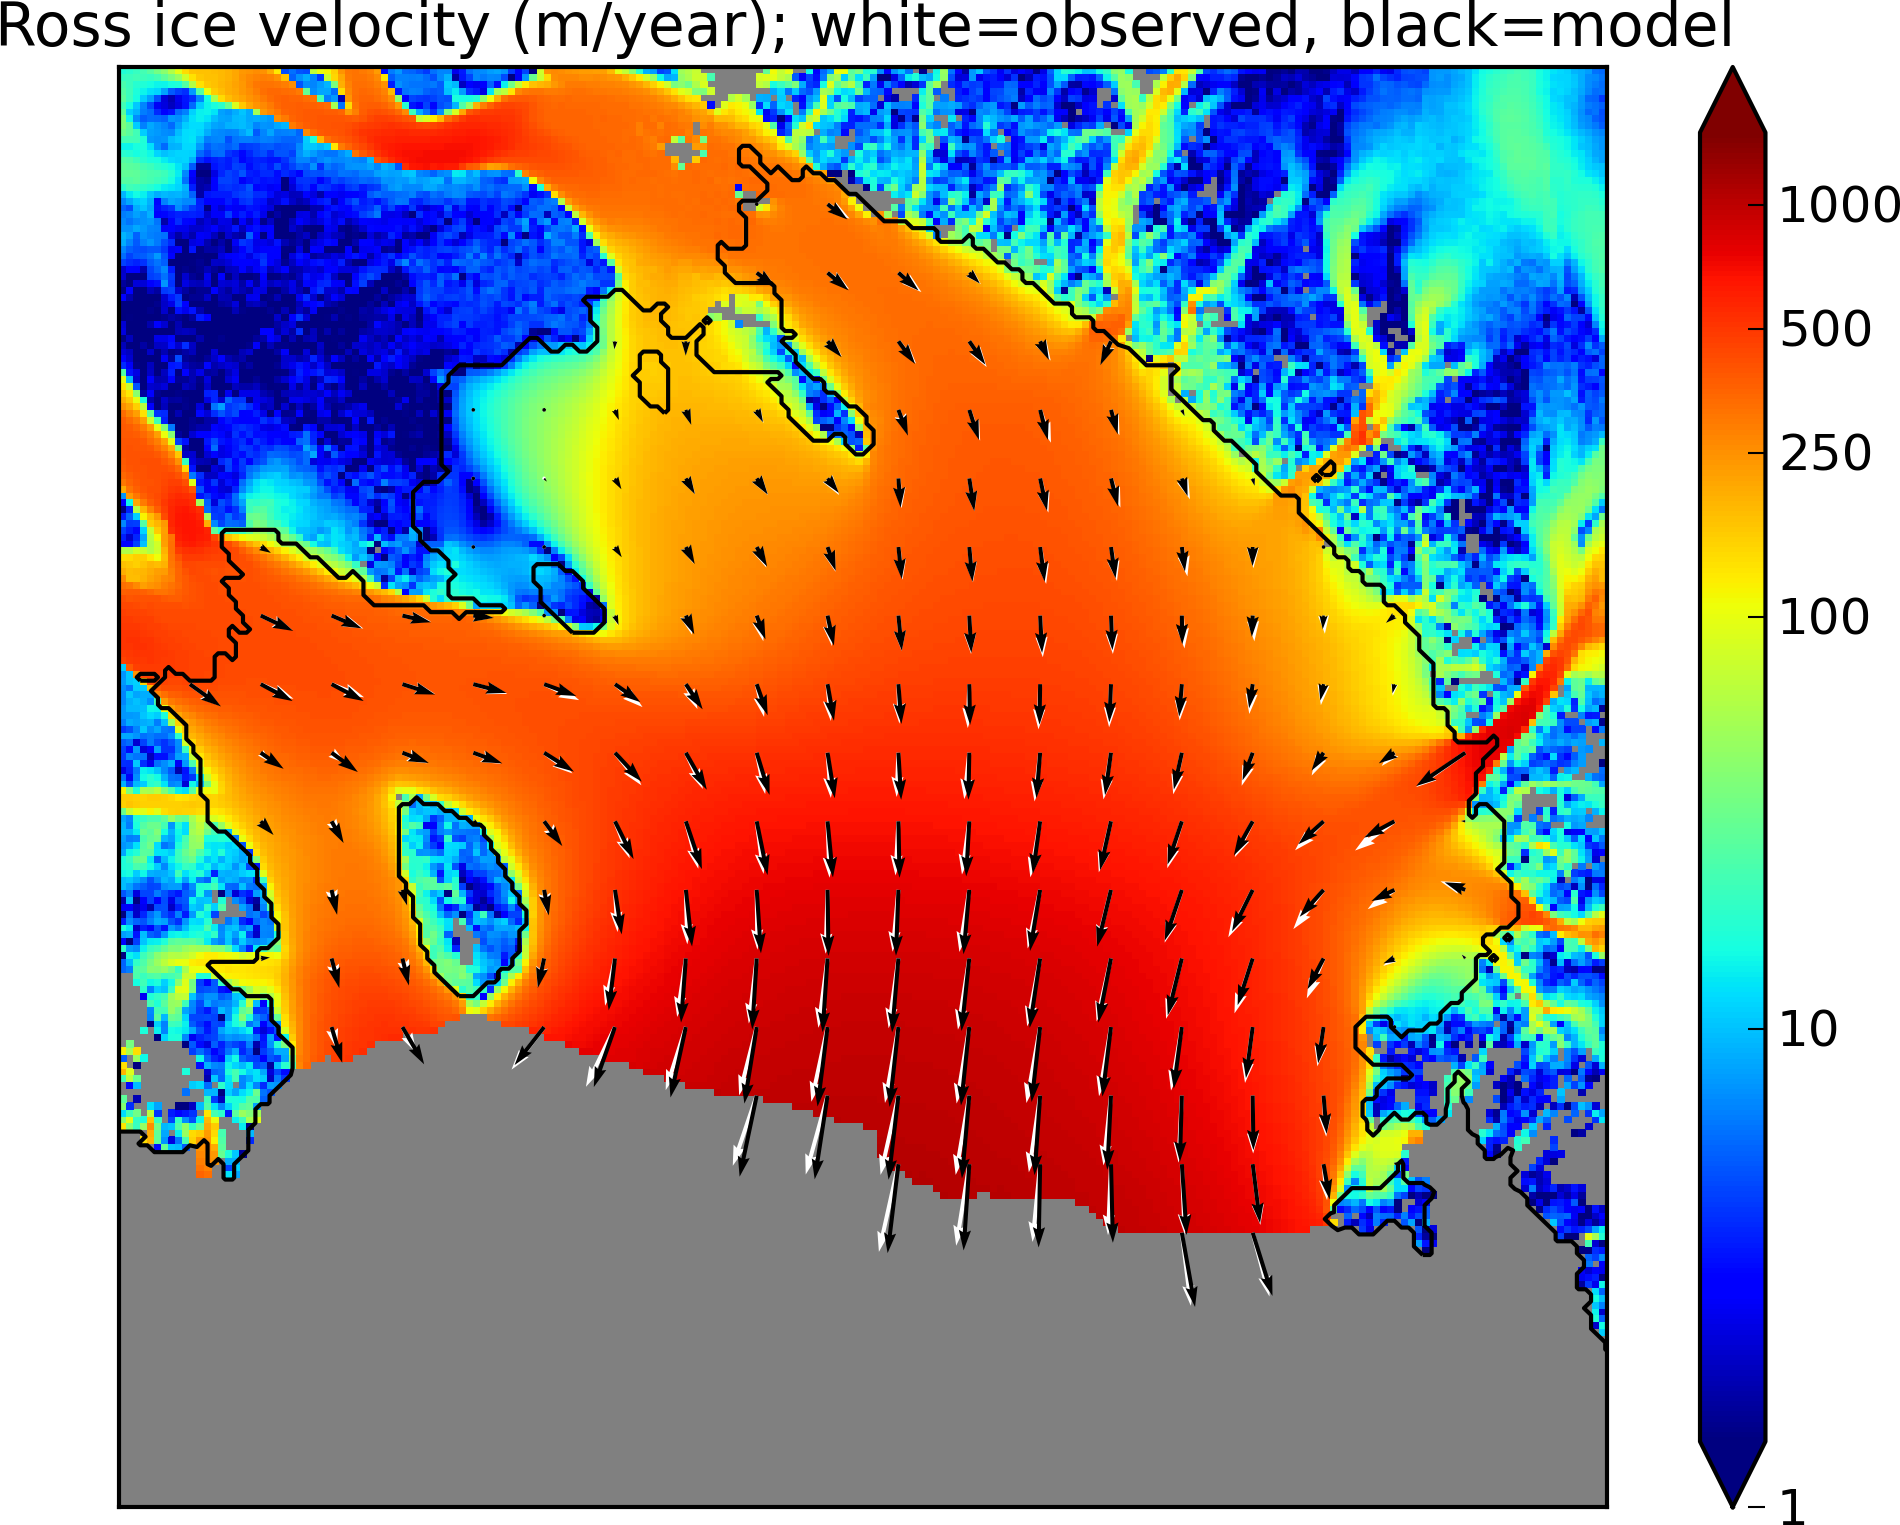
\includegraphics[width=3.3in,keepaspectratio=true]{rossquiver}\quad 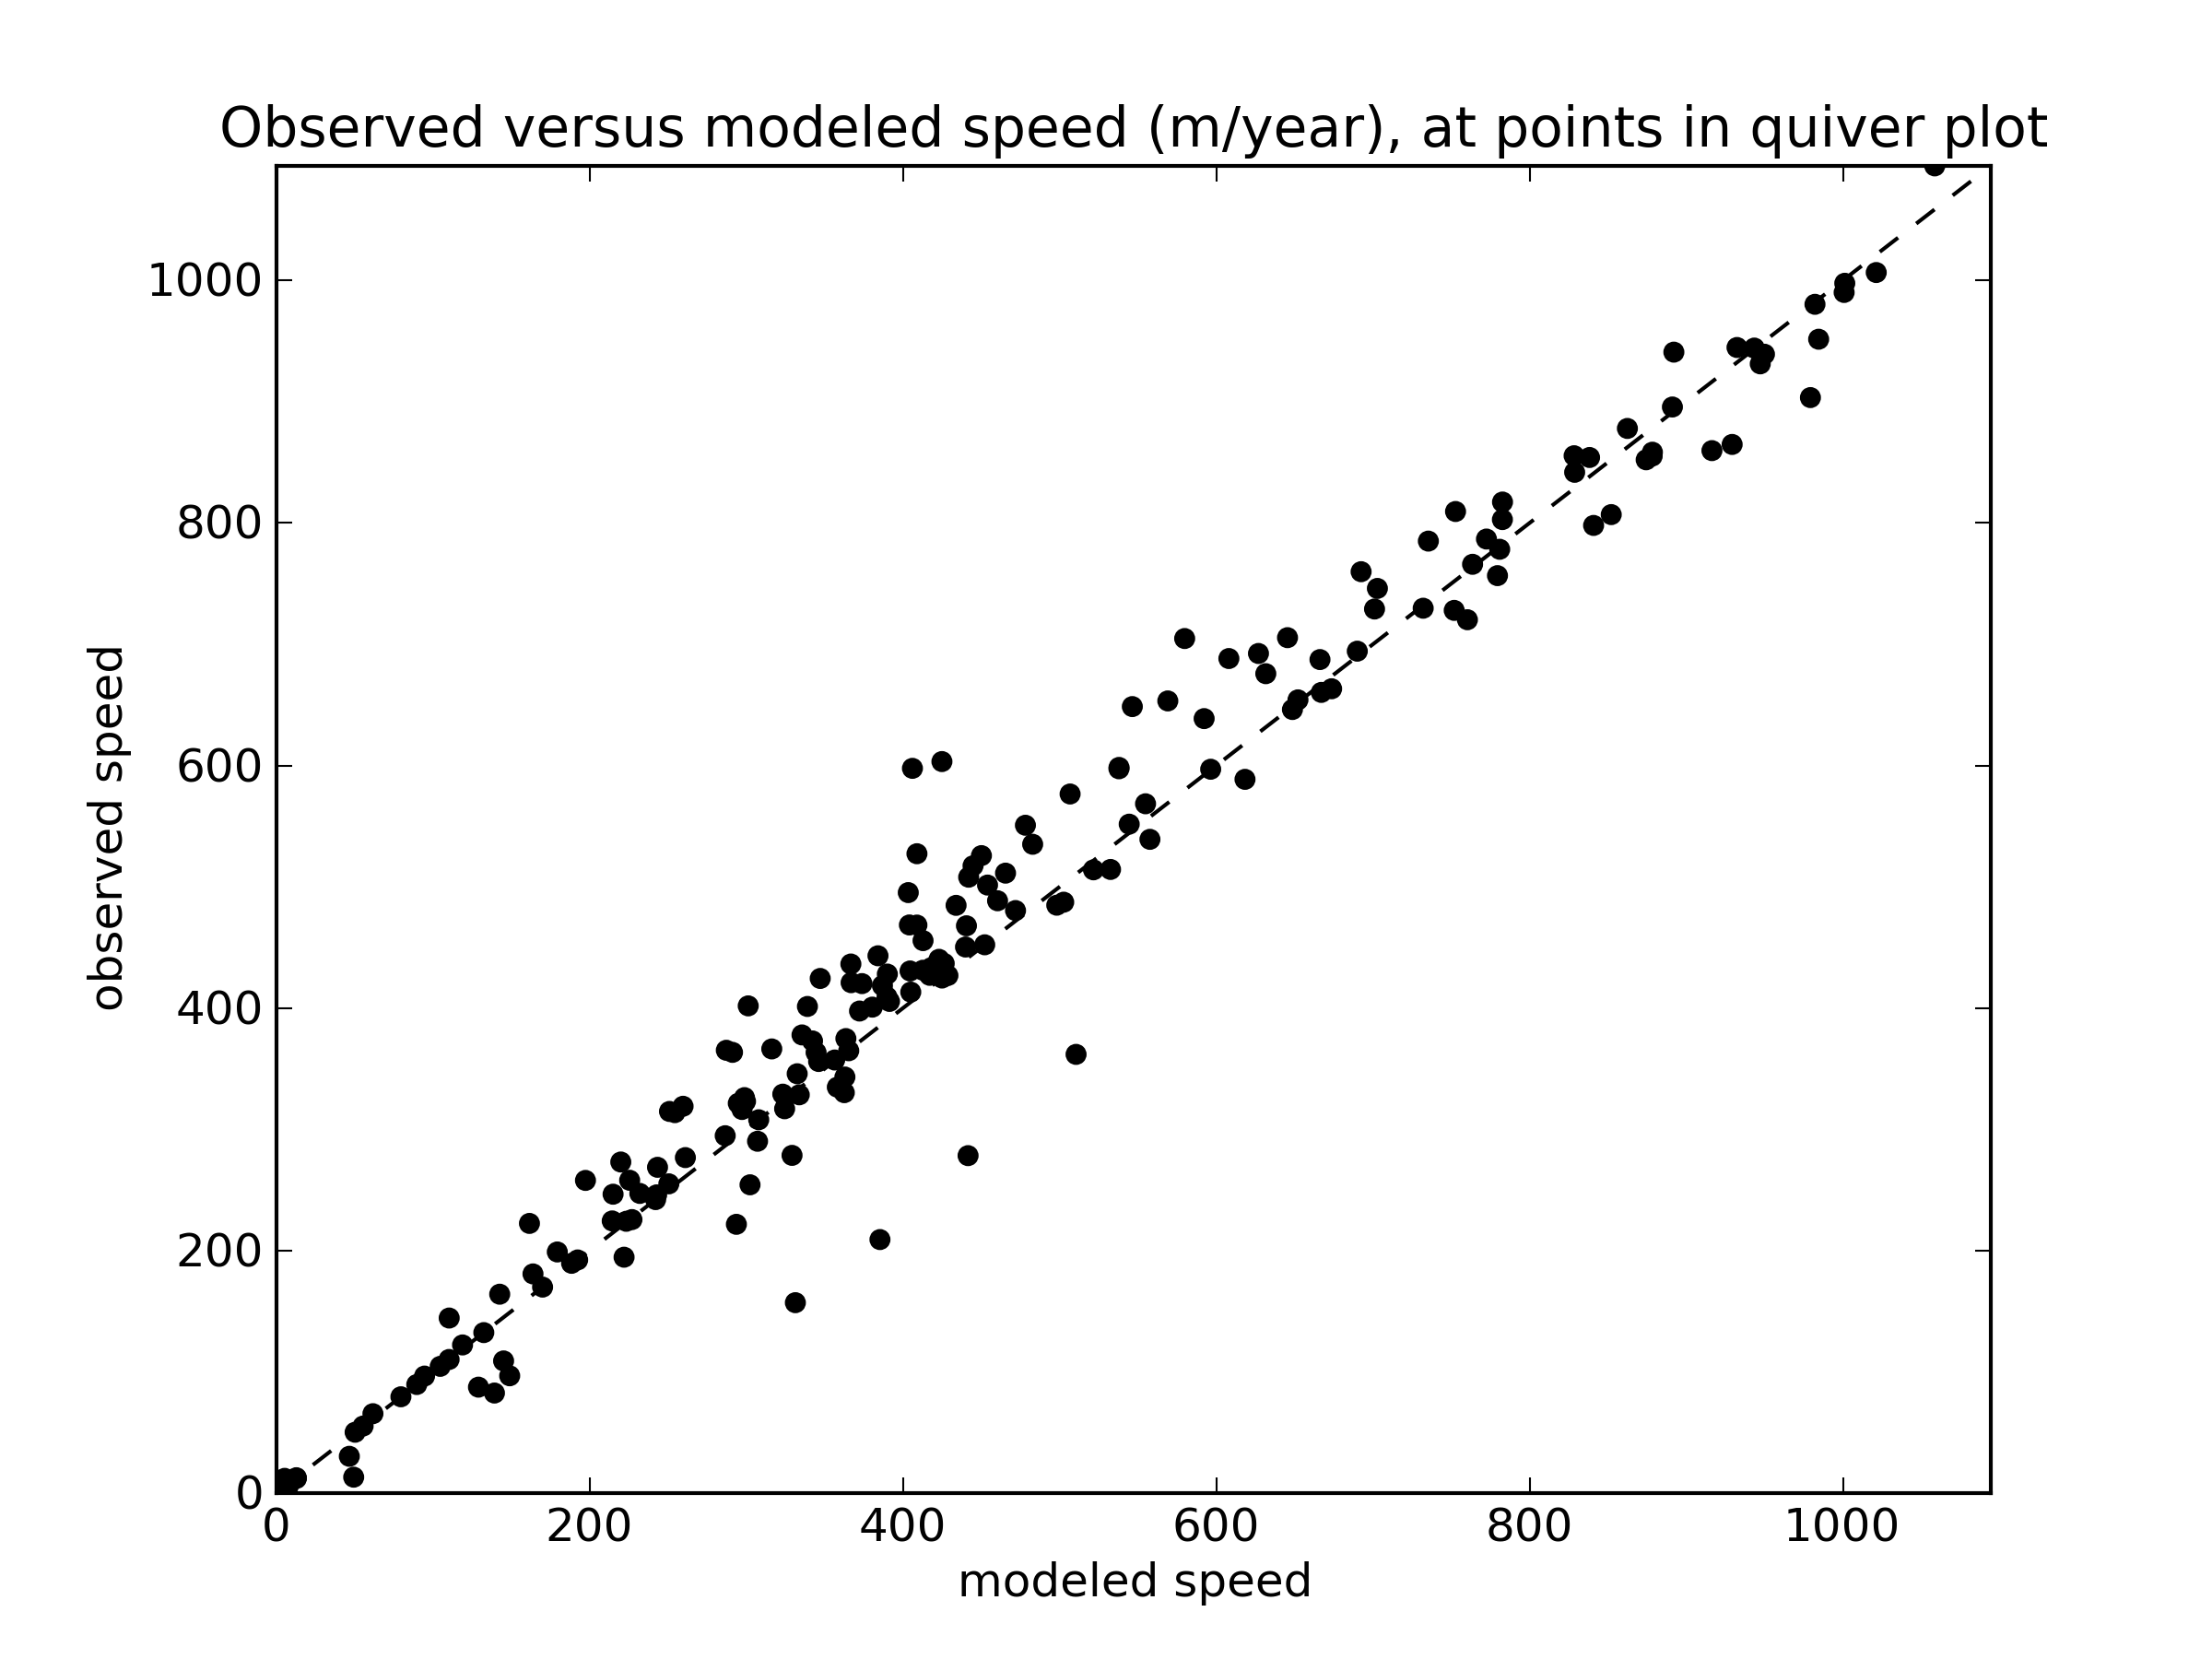
\includegraphics[width=2.7in,keepaspectratio=true]{rossscatter}}
\caption{\protect{\emph{Left}}: Color is speed in m/a.  Arrows are observed (white) and modeled (black) velocities.  \protect{\emph{Right}}: Comparison between modeled and observed speeds at points plotted on the left; compare to Figure \ref{fig:eisrosspython}.}
\label{fig:rosspython}
\end{figure}

\begin{figure}[ht]
\centering
\mbox{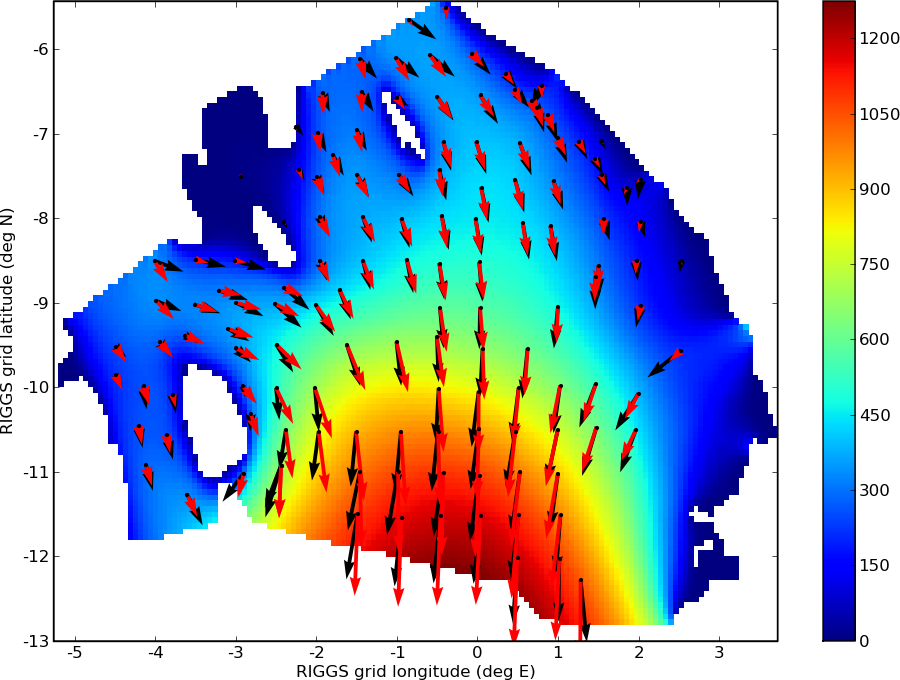
\includegraphics[width=3.3in,keepaspectratio=true]{oldeismintrossquiver}\quad 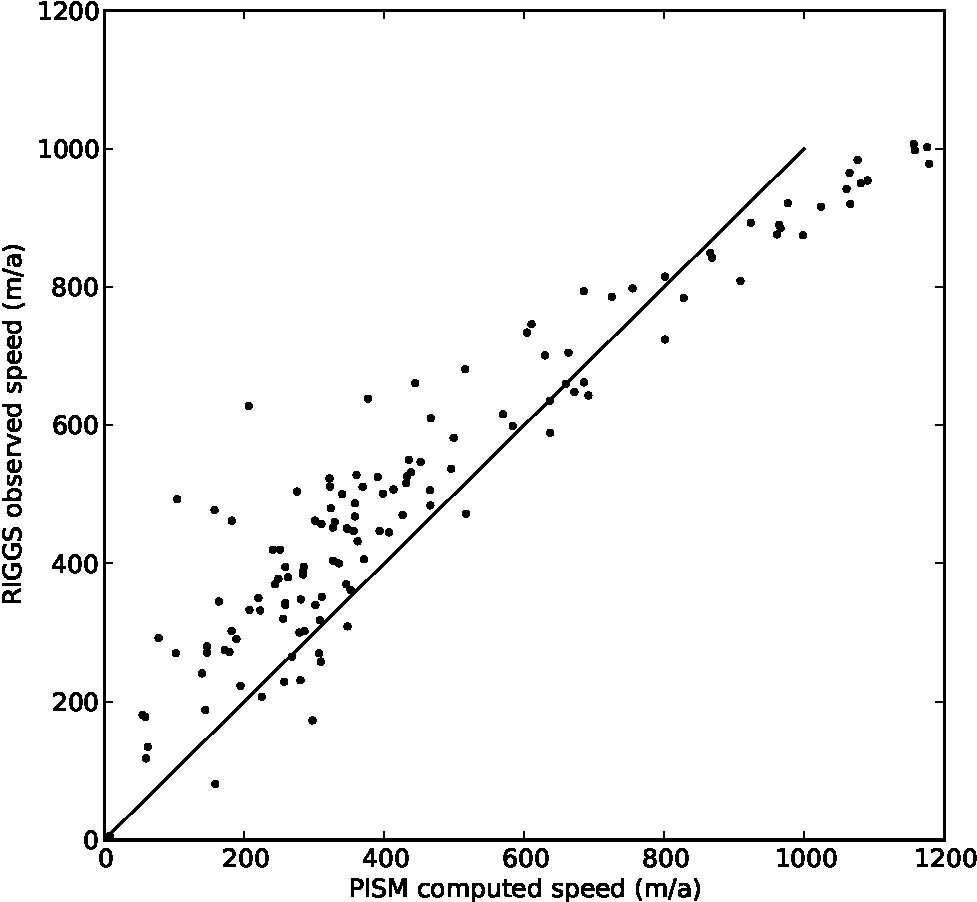
\includegraphics[width=2.7in,keepaspectratio=true]{oldeismintrossscatter}}
\caption{\protect{\emph{Left}}: Color is speed in m/a.  Arrows are observed (black) and computed (red) velocities at RIGGS points.  \protect{\emph{Right}}: Comparison between modeled and observed speeds at RIGGS points; compare Figure 2 in \cite{MacAyealetal}.}
\label{fig:eisrosspython}
\end{figure}

\subsubsection*{Extending this example}

The mechanism described in this section can be easily extended to create flow models of Filchner-Ronne Ice Shelf as in \cite{AlbrechtLevermann2012}, for example. All you need is choose a different part of the domain covered by data-sets used here. See \texttt{preprocess.py} for details.

One can also create a \emph{dynamical} model if an ice shelf with constant-in-time inflow from the grounding line. See scripts in \texttt{examples/ross/prognostic}.

%%% Local Variables:
%%% mode: latex
%%% TeX-master: "manual"
%%% End:
